
%*******************************************************************************
%*********************************** Second Chapter ***************************
%*******************************************************************************
%!TEX root = 0.main.tex

\section{Other samplings and other Discrete Laplacians}

[What we want from the Laplacian matrix]\\
In a Graph Spherical CNN we use the fact that when the sampling of the sphere is regular enough, the graph $W_{i j} = \exp {-\frac{\norm{x_i-x_j}^2}{4t}}$ is such that the corresponding graph Laplacian $\mathbf L_n^t=D-W$ has a spectrum that is close enough to the spectrum of $\triangle$ so that we can approximate a spherical convolution of a signal with a kernel with a multiplication of a polynomial of the discrete Laplacian $\sum_k \theta_k (\mathbf L_n^t)^k$ times the vector of the sampled signal $\mathbf f_i = f(x_i)$. 

[Stating the problem we want to solve]\\
In Chapter 2 we showed a way to construct $\mathbf L_n^t$ that well approximates $\triangle$ in the case of a much regular sampling of the sphere, HEALPix. In this Chapter we focus to others samplings less uniform than HEALPix. The sampling that we will use for our study, very used in applications, is the so called equiangular sampling. We will observe that in this case the Heat Kernel Graph Laplacian matrix is not able to correctly approximate the continuous Laplace-Beltrami operator, due to the fact that the equiangular sampling samples some specific areas of the sphere more than others. The goal of this chapter is to find a way of building a discrete approximation $\mathbf L$ of the Laplace-Beltrami operator more robust to non uniform sampling than the Heat Kernel Graph Laplacian matrix $\mathbf L_n^t$ used so far.

[Say what we did to solve it]\\
This chapter is organized as follows: In Section \ref{sec:Chapter3: Heat Kernel Graph Laplacian on the Equiangular Sampling} we introduce the equiangular sampling and the results that we obtained with the Heat Kernel Graph Laplacian matrix. In Section \ref{sec:Chapter3: other discrete laplacians} we present a short overview of different ways of building an discrete approximation of the Laplace-Beltrami operator; in Section \ref{sec:Chapter3: Using the Finite Element Method to approximate the Laplace-Beltrami operator on a manifold} we deepen how to use the Finite Element Method (FEM) to construct a discrete approximation of $\triangle$ and how this way of constructing $\mathbf L$  is actually capable of taking into account the non uniformity of the sampling and correct it. in Section \ref{sec:Chapter3: Results} we present and discuss the results obtained.
\subsection{Heat Kernel Graph Laplacian on the Equiangular Sampling}
\label{sec:Chapter3: Heat Kernel Graph Laplacian on the Equiangular Sampling}

\subsubsection{The Equiangular Sampling}
[Present the equiangular sampling]\\
Given the usual parametrization $x = x(\theta, \phi)$ of the sphere
$$
\mathbb{S}^{2}=\left\{x=\left(x_{1}, x_{2}, x_{3}\right) \in \mathbb{R}^{3} :\|x\|_{\mathbb{R}^{3}}=\left(x_{1}^{2}+x_{2}^{2}+x_{3}^{2}\right)^{1 / 2}=1\right\}
$$

$$
x_{1}=\cos (\phi) \sin (\theta), \quad x_{2}=\sin (\phi) \sin (\theta), \quad x_{3}=\cos (\theta)
$$
Let $m\in\mathbb N$, the uniform sampling of bandwidth $b=2^m$ is given by 
$
x_{j k}^{(b)}=x\left(\theta_{j}^{(b)}, \phi_{k}^{(b)}\right)
$
where
$$
\theta_{j}^{(b)} :=\pi \frac{j}{2 b}, \quad \phi_{k}^{(b)} :=2 \pi \frac{k}{2 b}
$$
\begin{figure}[h!]
	\centering
	\label{fig:equiangular sampling}
	\caption{Equiangular sampling with bandwidth $n=16$}
	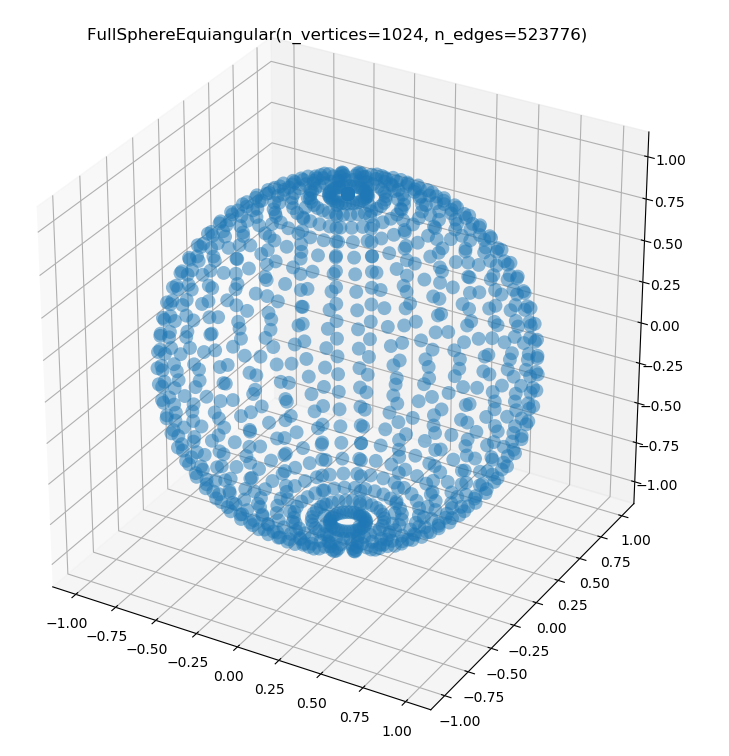
\includegraphics[width=0.5\textwidth]{../codes/02.HeatKernelGraphLaplacian/equiangular/equiangular.png}
\end{figure}
One has $n=4b^2$ points on the sphere, where $x_{0 k}^{(b)}$ corresponds to the north pole for every $k$. Notice also that the south pole is never sampled. In figure \ref{fig:equiangular sampling} it can also be appreciated how the area close to the poles is much more sampled that the equator. One reason for which this sampling is very useful is the following result from \cite{Driscoll:1994:CFT:184069.184073}, that states that any band limited function can be exactly recovered from its sampled values $f\left(x_{j k}^{(b)}\right)$:
\vspace{0.5cm}
\begin{prop}\label{prop:equiangular sampling theorem}
	Let \(l_{0} \in \mathbb{N}\) and \(m_{0} \in \mathbb{Z},\left|m_{0}\right| \leq l_{0} .\) If \(f=\sum_{l=0}^{b-1} \sum_{m=-l}^{l} \widehat{f}(l, m) Y_{l}^{m}\)
	then
	
	$$
	\begin{aligned} \widehat{f}\left(l_{0}, m_{0}\right)=& \frac{1}{4 b^{2}} \sum_{j=0}^{2 b-1} \sum_{k=0}^{2 b-1} f\left(x_{j k}^{(b)}\right) \overline{Y_{l_{0}}^{m_{0}}\left(x_{j k}^{(b)}\right)} \sin \left(\theta_{j}^{(b)}\right) \times \\ & \times \frac{4}{\pi} \sum_{l=0}^{b-1} \frac{1}{2 l+1} \sin \left((2 l+1) \theta_{j}^{(b)}\right) \end{aligned}
	$$
\end{prop}
\vspace{0.5cm}

\subsubsection{Heat Kernel Graph Laplacian}
Thanks to Proposition \ref{prop:equiangular sampling theorem}, assuming we can compute the Fourier transform of the eigenvectors of the Heat Kernel Graph Laplacian matrix and see how much they are aligned with the eigenspaces of the true Laplace-Beltrami operator. Here the results:


\begin{table}[h!]
	\centering
	\label{table:equiangular kernel width}
	\caption{Kernel width $t$ used to construct the Heat Kernel Graph Laplacian matrix fr each bandwidth $b$}
	\begin{tabular}{ c|c } 
	
$b$ & $t$ \\ 
	\hline
4 & 0.5 \\ 
8 & 0.3 \\ 
16 & 0.1 \\ 
	
	\end{tabular}
\end{table}

\begin{figure}[h!]
	\centering
	\label{fig:equiangular sampling alignment}
	\caption{Alignment of eigenspaces of the Heat Kernel Graph Laplacian matrix with the true Laplace-Beltrami eigenspaces on the equiangular sampling with $b=16$ and kernel width $t=0.1$}
	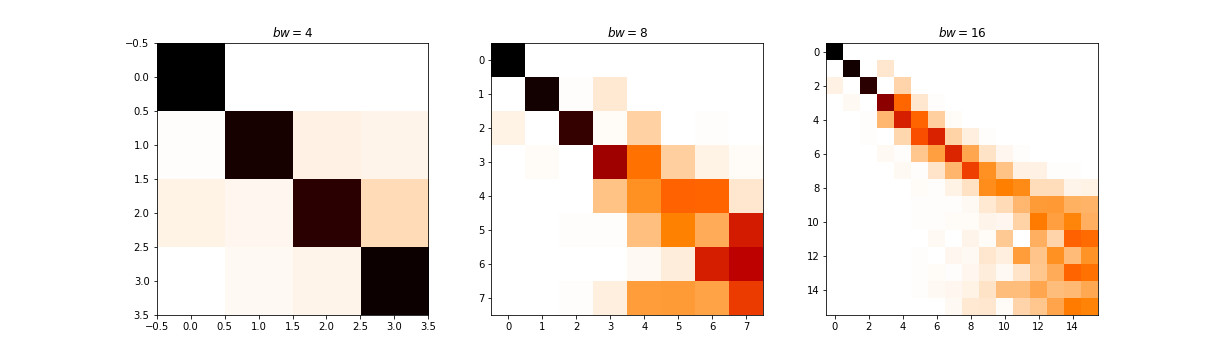
\includegraphics[width=0.9\textwidth]{../codes/02.HeatKernelGraphLaplacian/equiangular/equi_full.png}
\end{figure}
\begin{figure}[h!]
	\centering
	\label{fig:equiangular sampling alignment diagonal}
	\caption{Alignment of eigenspaces of the Heat Kernel Graph Laplacian matrix with the true Laplace-Beltrami eigenspaces on the equiangular sampling}
	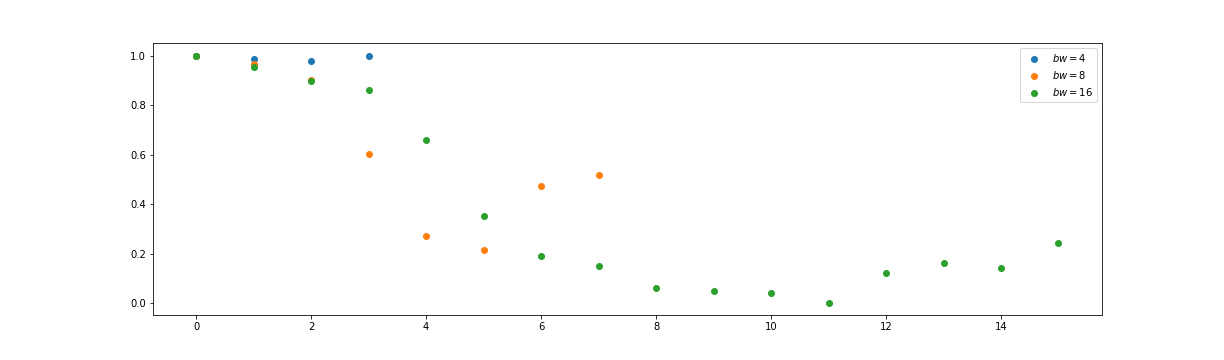
\includegraphics[width=0.9\textwidth]{../codes/02.HeatKernelGraphLaplacian/equiangular/equi_full_diagonal.png}
\end{figure}
\begin{figure}[h!]
	\centering
	\label{fig:equiangular sampling alignment eigenvalues}
	\caption{Eigenvalues of the Heat Kernel Graph Laplacian matrix on the equiangular sampling with $b=16$ and kernel width $t=0.1$}
	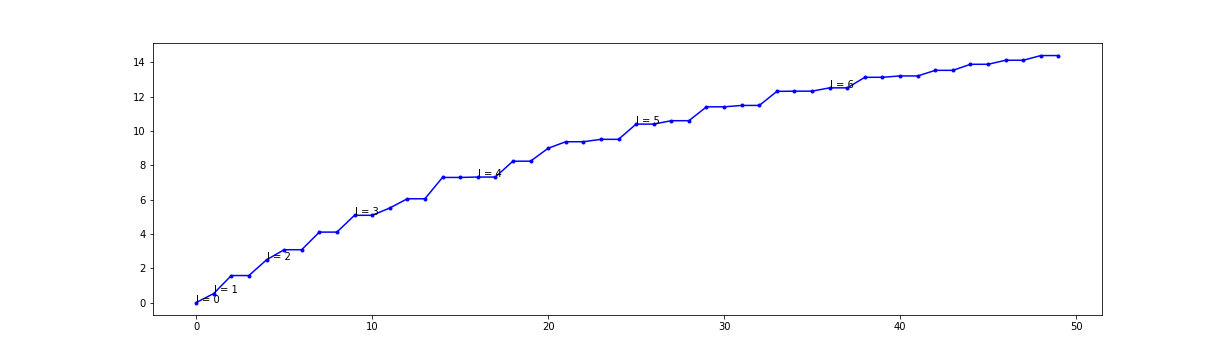
\includegraphics[width=0.9\textwidth]{../codes/02.HeatKernelGraphLaplacian/equiangular/equi_full_eigenvalues_16.png}
\end{figure}

It can be appreciated how poor these results are compared to the ones obtained with the HEALPix sampling. \\

[ Explain why they are so bad: Perspective of the quadrature formula]\\
A way to understand what's going on is the following: remembering the proof of theorem \ref{theo:pointwise convergence in the healpix case} and using again the notation $\phi^{t}(x ; y)=e^{-\frac{||x-y||^2}{4t}}\left(f(y)-f(x)\right)$, the key thing is to make $L_n^tf(y)=\sum_i \frac{1}{n} \phi^{t}(x_i ; y)$  approximate $L^tf(y)=\int_\mathcal M\phi^{t}(x ; y)d\mu(x)$, in other words we can see the graph weights as \textit{quadrature weights} meant to approximate the continuous integral on the right hand side of equation \ref{eq:quadrature approximation}.
\begin{equation}
\label{eq:quadrature approximation}
	\sum_i \frac{1}{n} \phi^{t}(x_i ; y) \quad \approxeq\quad \int_\mathcal M\phi^{t}(x ; y)d\mu(x)
\end{equation}
The way of building the graph of Belkin et al. works in the case of random sampling because in that way the sampling in the limit of the SLLN will sample the manifold uniformly, and thus there's no need of re-weighting the graph; in case of non uniform sampling, we intuitively need to modify the Heat Kernel weights $W_{i j}=e^{-\frac{\norm{x_i-x_j}^2}{4t}}$ with some coefficients $\alpha_i$ to create a re-weighted graph 
$$
W'_{i j} = \alpha_i W_{i j}
$$

in order for $L_n^tf(y)$ to correctly approximate $L^tf(y)$, where $\alpha_i$ would be smaller in pixels that are in areas closer to the poles and bigger in areas closer to the equator. 

\begin{equation}
\label{eq:quadrature approximation 2}
\sum_i \frac{1}{n} \alpha_i \phi^{t}(x_i ; y) \quad \approxeq\quad \int_\mathcal M  \phi^{t}(x ; y)d\mu(x)
\end{equation}
In the next section we present some different ways of building the matrix $\mathbf L$.

\clearpage
\subsection{Other Discrete Laplacians}\label{sec:Chapter3: other discrete laplacians}
Present all the other ways of approximating the Laplace-Beltrami operator you found: graphs, Laplace de Rham, FEM
\subsection{Using the Finite Element Method to approximate the Laplace-Beltrami operator on a manifold}\label{sec:Chapter3: Using the Finite Element Method to approximate the Laplace-Beltrami operator on a manifold}
Basic ingredients: works on a mesh, 
\subsubsection{Galerkin Method and Finite Element Method}
General introduction to the FEM: definitions, weak formulation, functional spaces, Galerkin method, linear FEM.
\subsubsection{The eigenvalue problem on a manifold}
Weak formulation of the eigenvalue problem on the sphere, generalized eigenvalue problem, lumping of the mass matrix, discussion on the solvers
\subsection{Results}
\label{sec:Chapter3: Results}
\begin{figure}[h]
	\label{fig:HeatKernelGraphLaplacianHealpix}
	\caption{Heat Kernel Graph Laplacian on HEALPix}
	\centering
	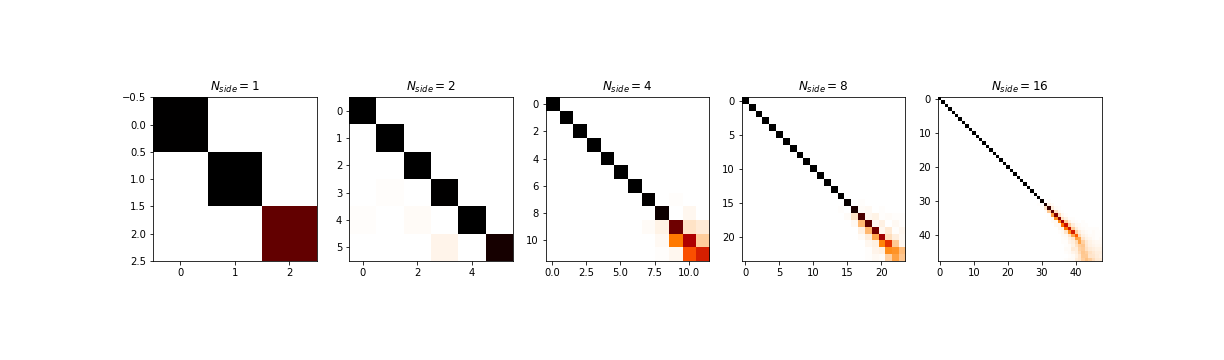
\includegraphics[width=0.9\textwidth]{../codes/02.HeatKernelGraphLaplacian/HEALPix/06_figures/optimal_thresholded.png}
	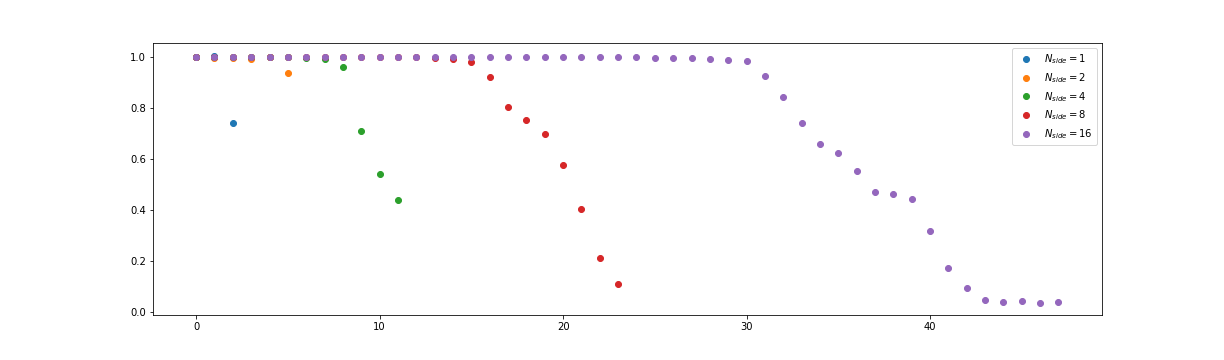
\includegraphics[width=0.9\textwidth]{../codes/02.HeatKernelGraphLaplacian/HEALPix/06_figures/optimal_thresholded_diagonal.png}	
\end{figure}

\begin{figure}[h]
	\label{fig:FEMHealpix}
	\caption{Linear FEM Laplacian on HEALPix}
	\centering
	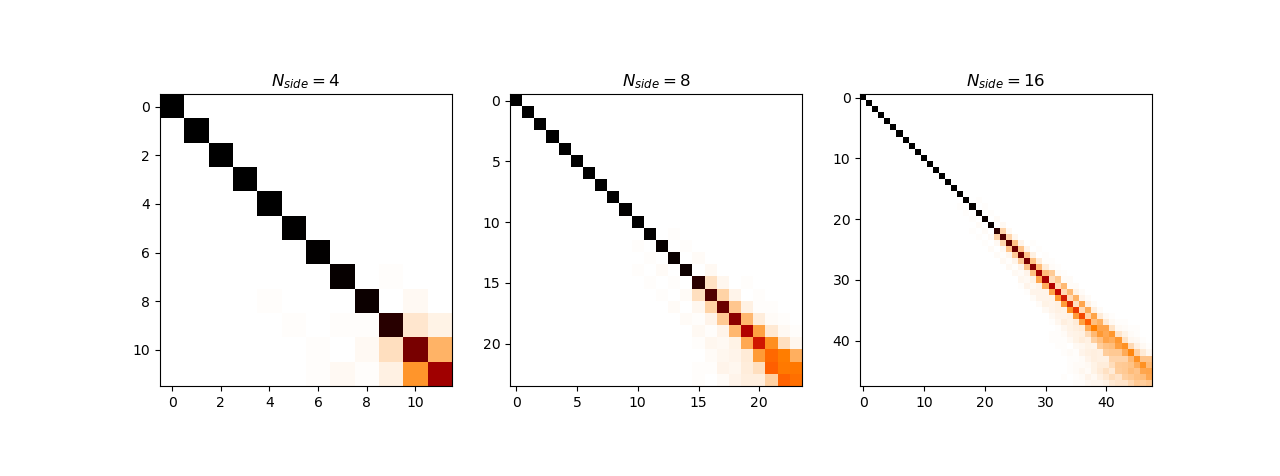
\includegraphics[width=0.8\textwidth]{../codes/03.FEM_laplacian/HEALPix/img/linearFEM.png}
	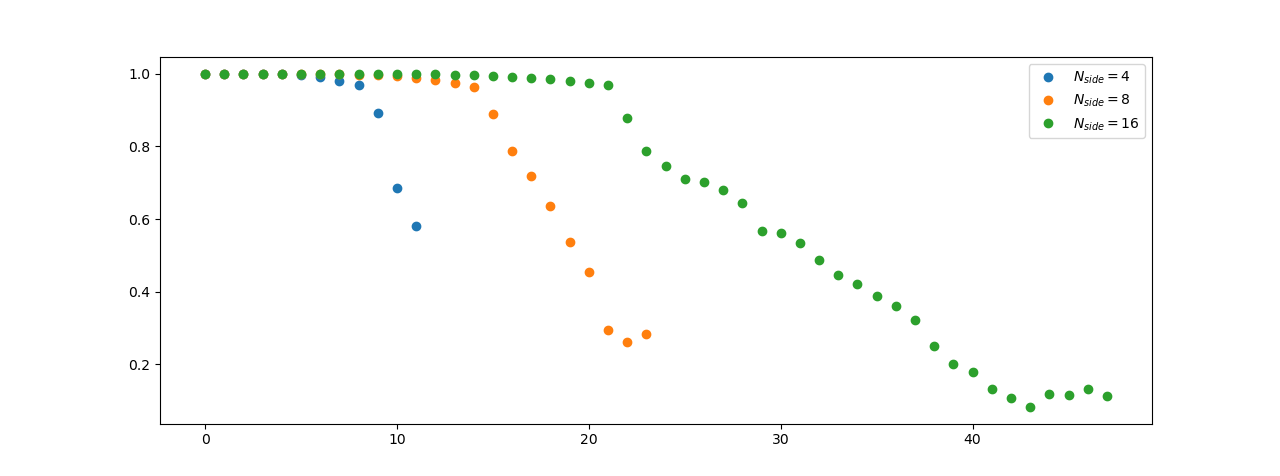
\includegraphics[width=0.8\textwidth]{../codes/03.FEM_laplacian/HEALPix/img/linearFEM_diagonal.png}	
	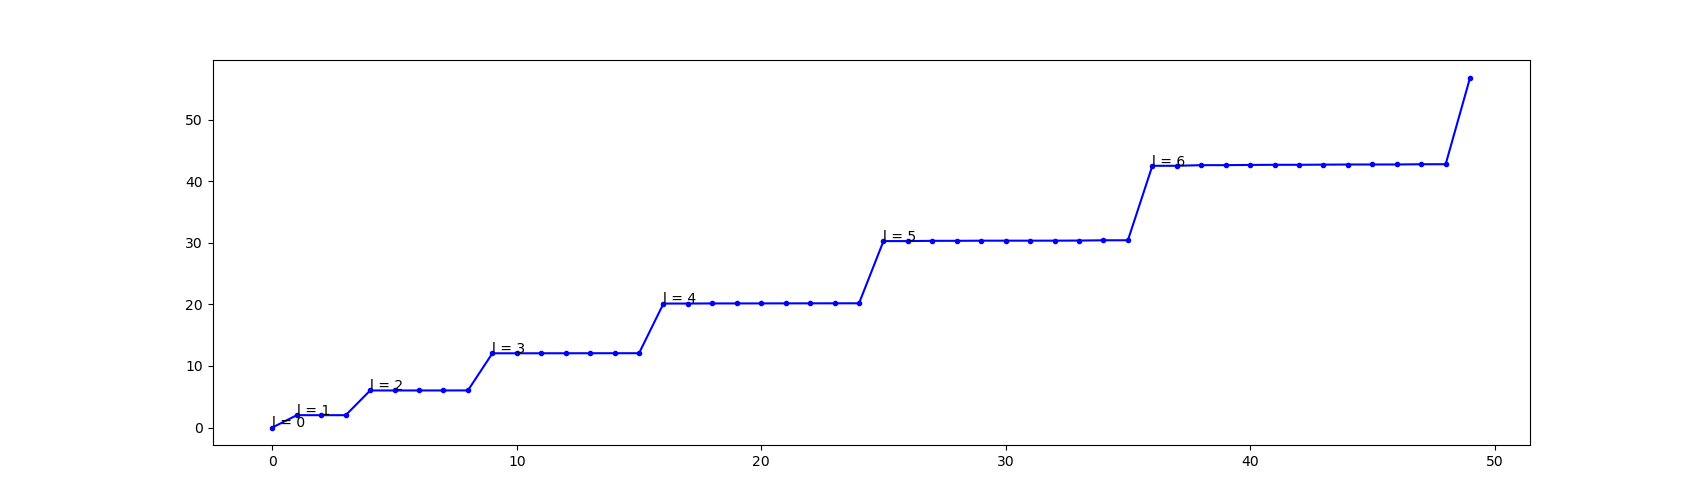
\includegraphics[width=0.8\textwidth]{../codes/03.FEM_laplacian/HEALPix/img/FEM_eigenvalues_16.png}	 
\end{figure}

\begin{figure}[h]
	\label{fig:FEM and graph diffusion on HEALPix}
	\caption{FEM and HKGL diffusion on HEALPix}
	\centering
	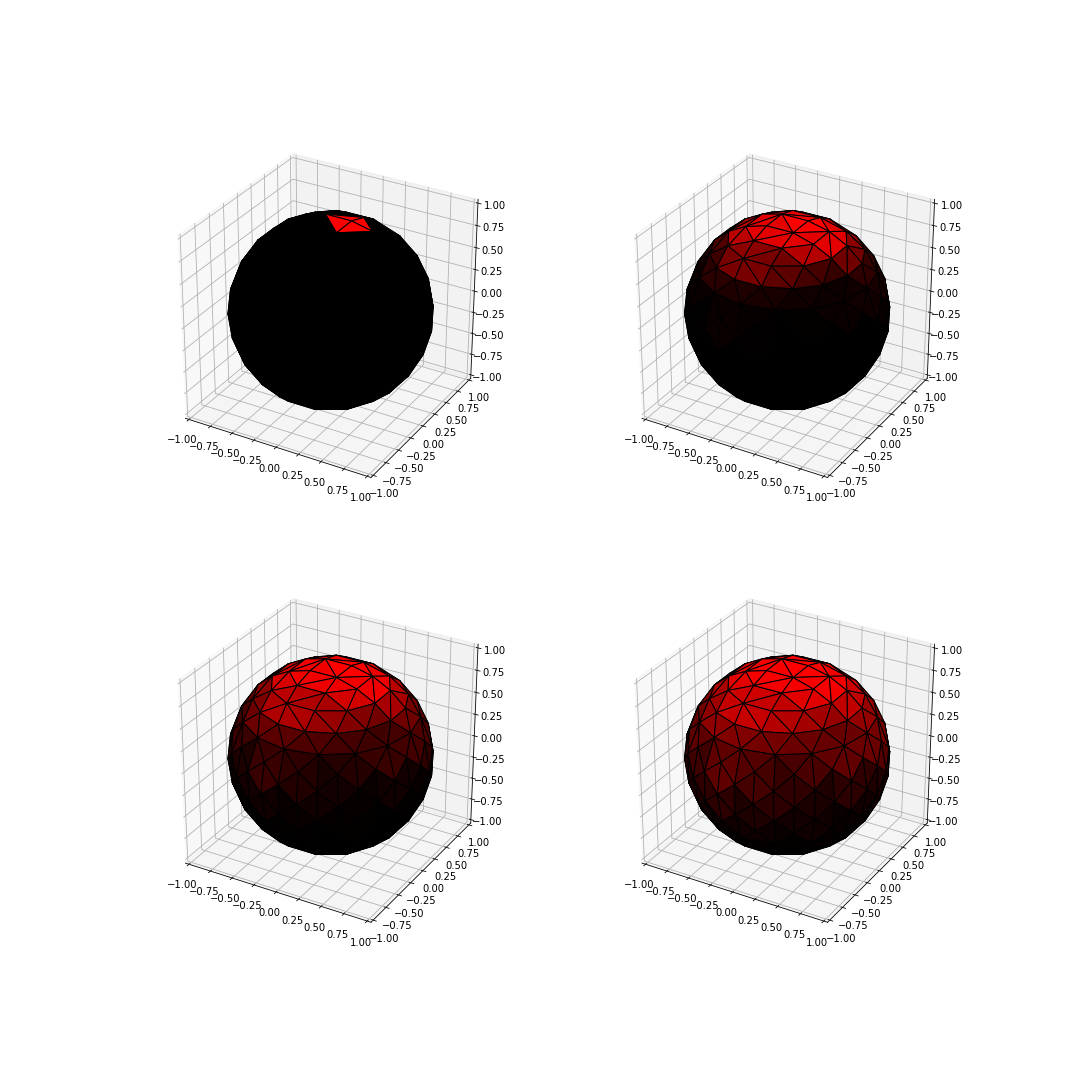
\includegraphics[width=0.6\textwidth]{../codes/03.FEM_laplacian/HEALPix/17_diffusion_img/FEM_diffusion.png}
	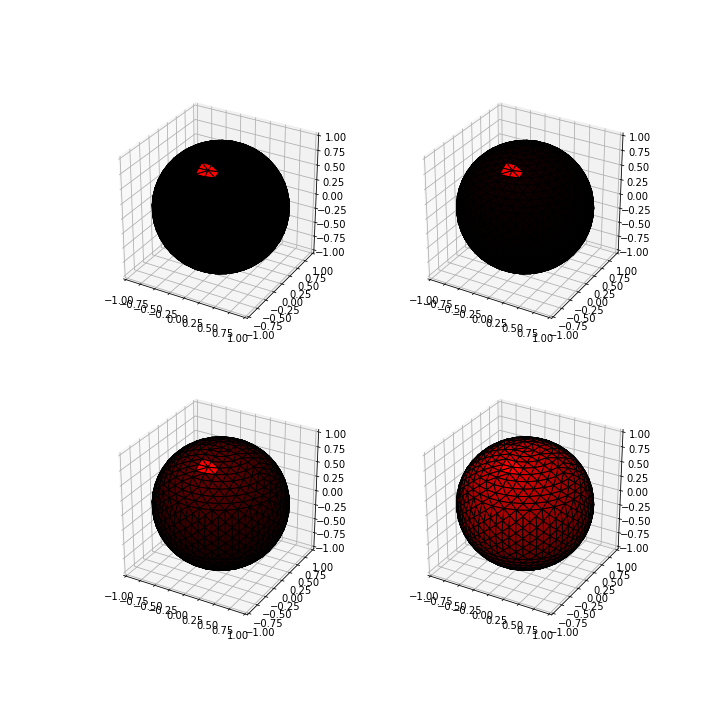
\includegraphics[width=0.6\textwidth]{../codes/03.FEM_laplacian/HEALPix/17_diffusion_img/GRAPH_diffusion.png}	

\end{figure}

\begin{figure}[h]
	\label{fig:HeatKernelGraphLaplacianEquiangular}
	\caption{Heat Kernel Graph Laplacian on equiangular sampling}
	\centering
	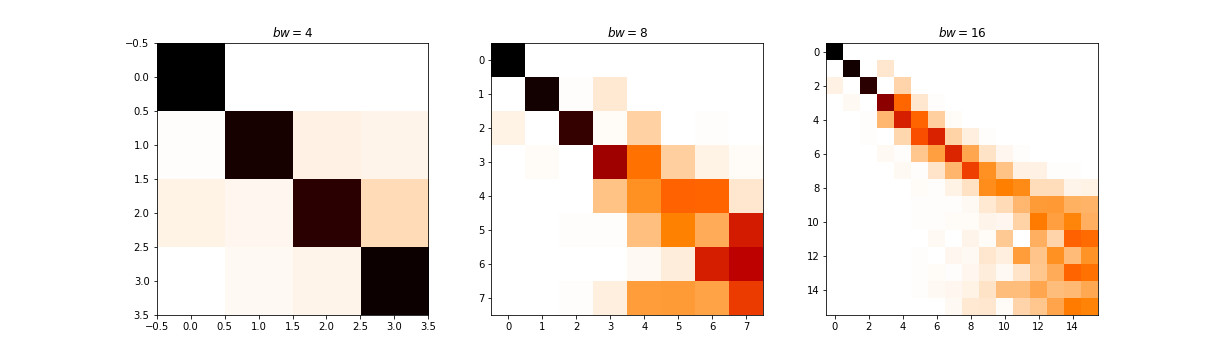
\includegraphics[width=0.9\textwidth]{../codes/02.HeatKernelGraphLaplacian/equiangular/equi_full.png}
	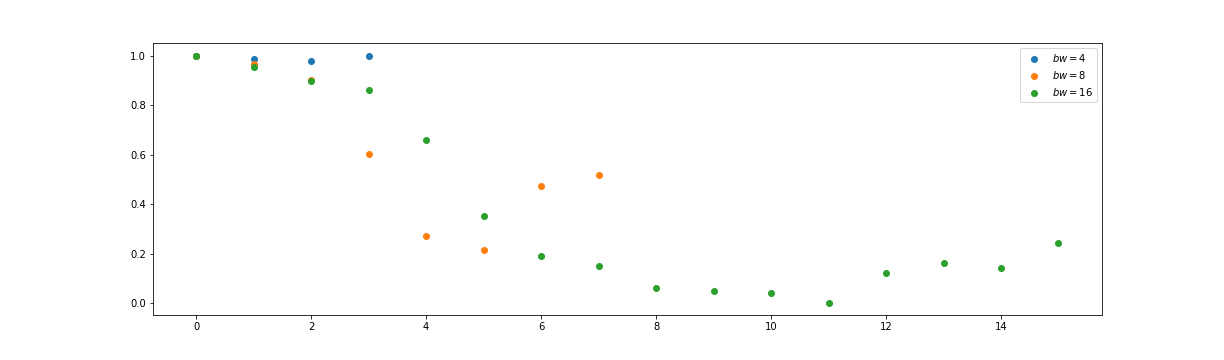
\includegraphics[width=0.9\textwidth]{../codes/02.HeatKernelGraphLaplacian/equiangular/equi_full_diagonal.png}	
	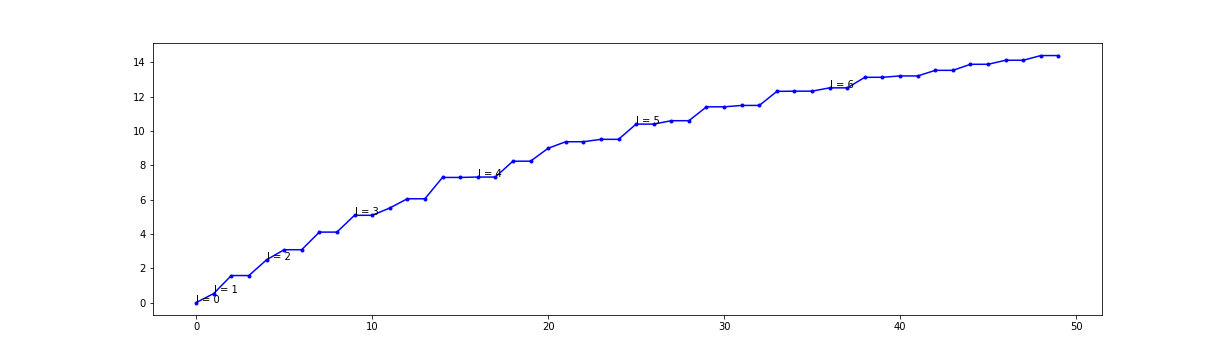
\includegraphics[width=0.9\textwidth]{../codes/02.HeatKernelGraphLaplacian/equiangular/equi_full_eigenvalues_16.png}	
\end{figure}

\begin{figure}[h]
	\label{fig:FEMequiangular}
	\caption{Linear FEM Laplacian on equiangular sampling}
	\centering
	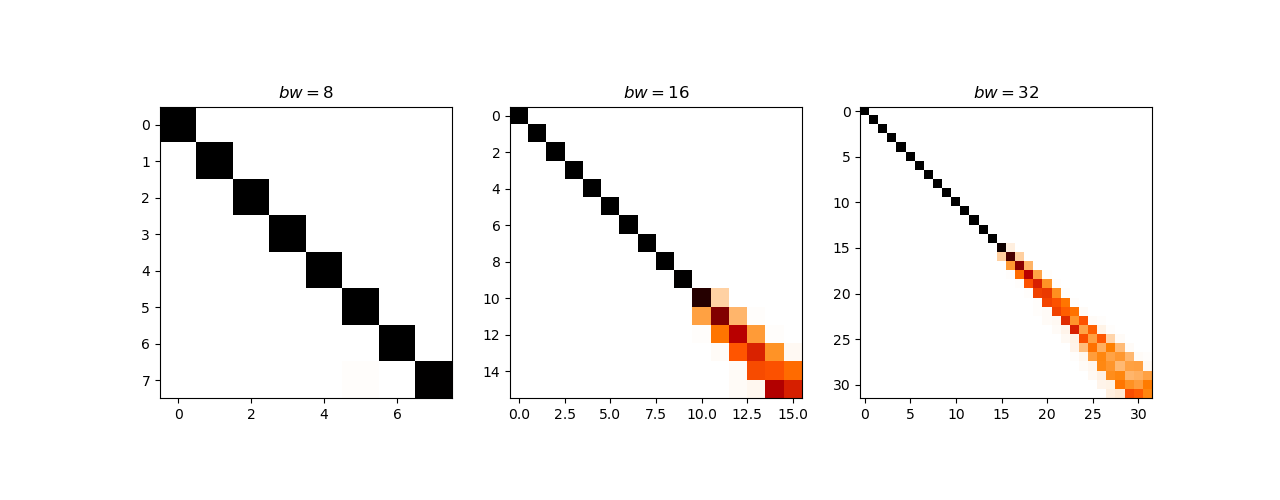
\includegraphics[width=0.9\textwidth]{../codes/03.FEM_laplacian/equiangular/normal/img/linearFEM.png}
	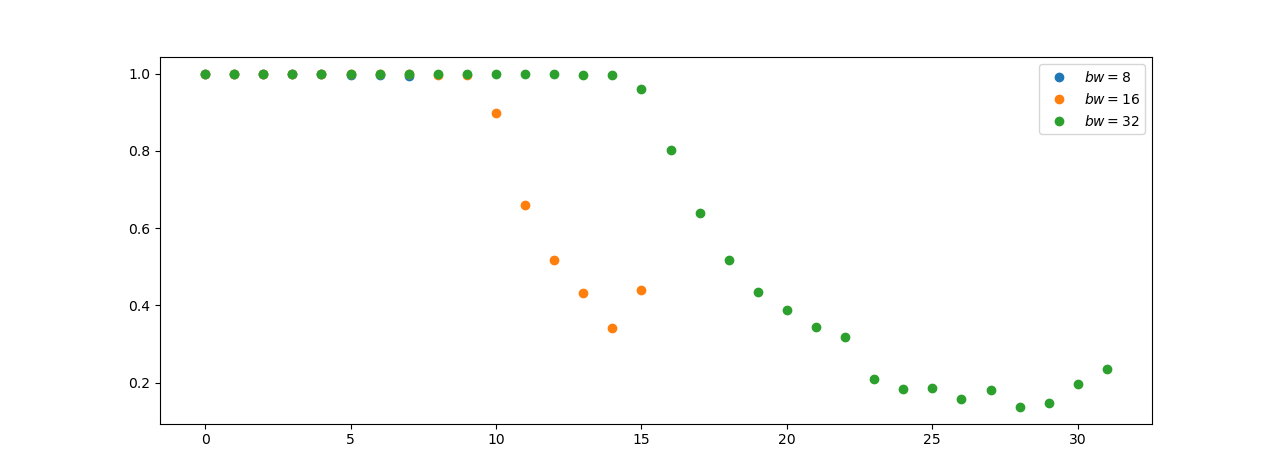
\includegraphics[width=0.9\textwidth]{../codes/03.FEM_laplacian/equiangular/normal/img/linearFEM_diagonal.png}	
	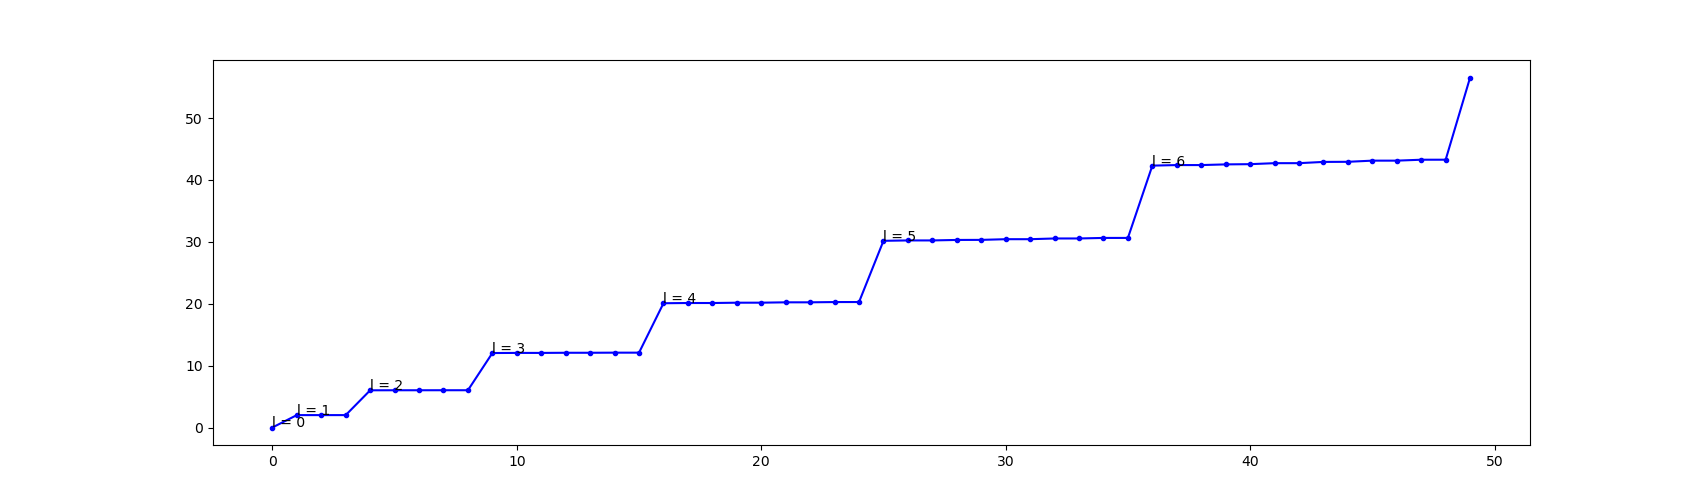
\includegraphics[width=0.9\textwidth]{../codes/03.FEM_laplacian/equiangular/normal/img/FEM_eigenvalues_16.png}	
\end{figure}

\begin{figure}[h]
	\label{fig:FEM and graph diffusion on equianular sampling}
	\caption{FEM and HKGL diffusion on equiangular sampling}
	\centering
	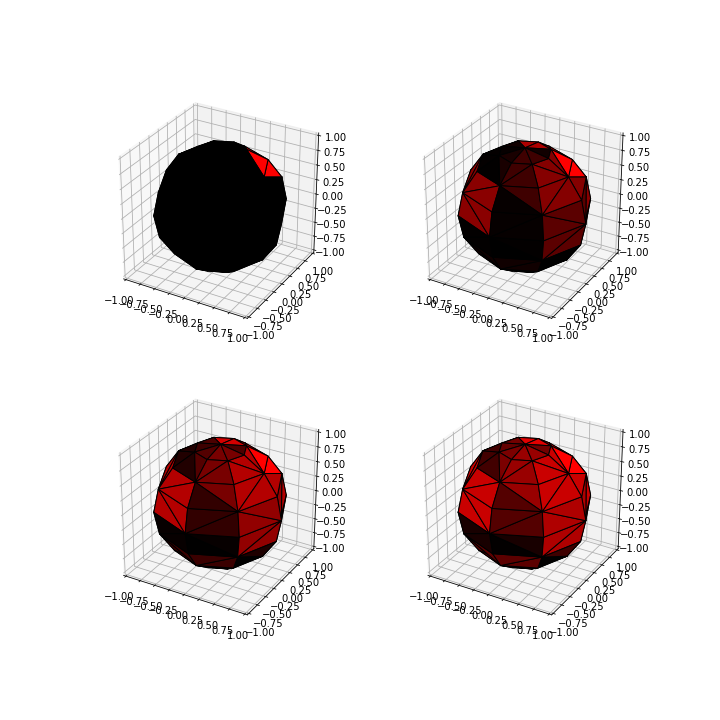
\includegraphics[width=0.6\textwidth]{../codes/03.FEM_laplacian/equiangular/normal/17_diffusion_img/FEM_diffusion.png}
	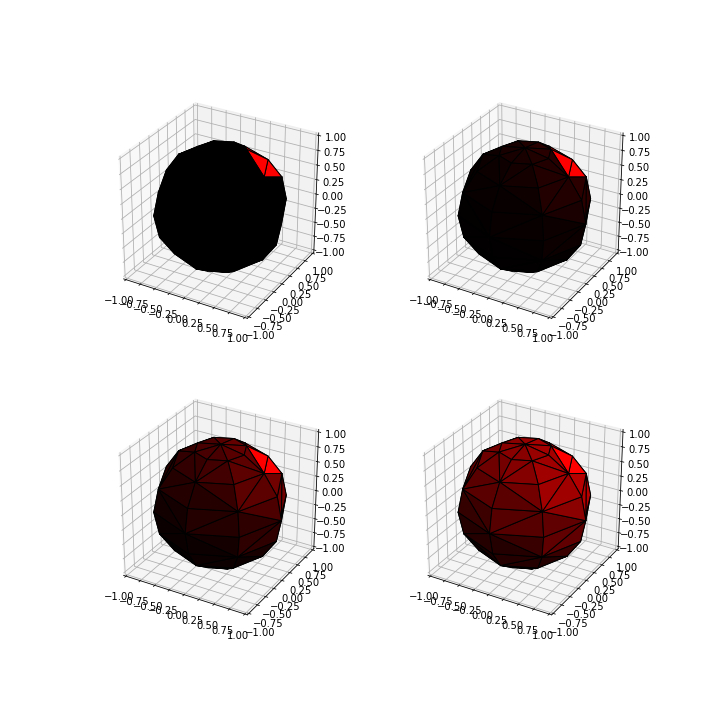
\includegraphics[width=0.6\textwidth]{../codes/03.FEM_laplacian/equiangular/normal/17_diffusion_img/GRAPH_diffusion.png}	
	
\end{figure}
\begin{figure}[h]
	\label{fig:FEMequiangularLumped}
	\caption{Lumped Linear FEM Laplacian on equiangular sampling}
	\centering
	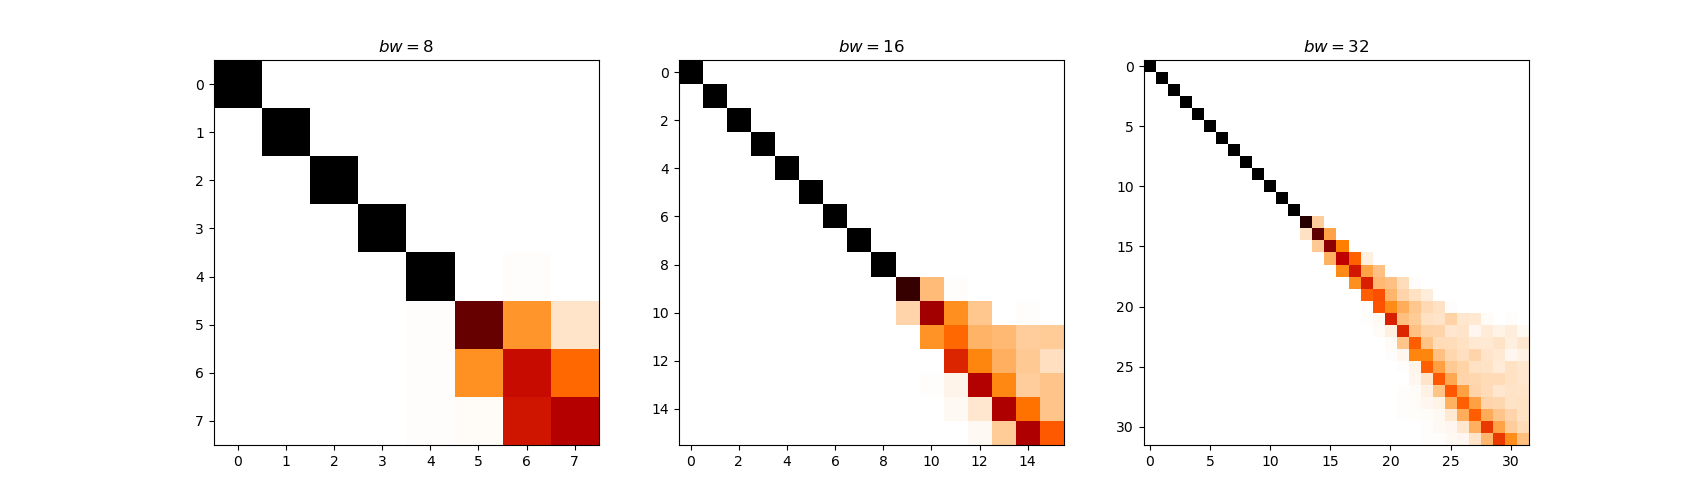
\includegraphics[width=0.9\textwidth]{../codes/03.FEM_laplacian/equiangular/mass_lumping/BL/img/linearFEM.png}
	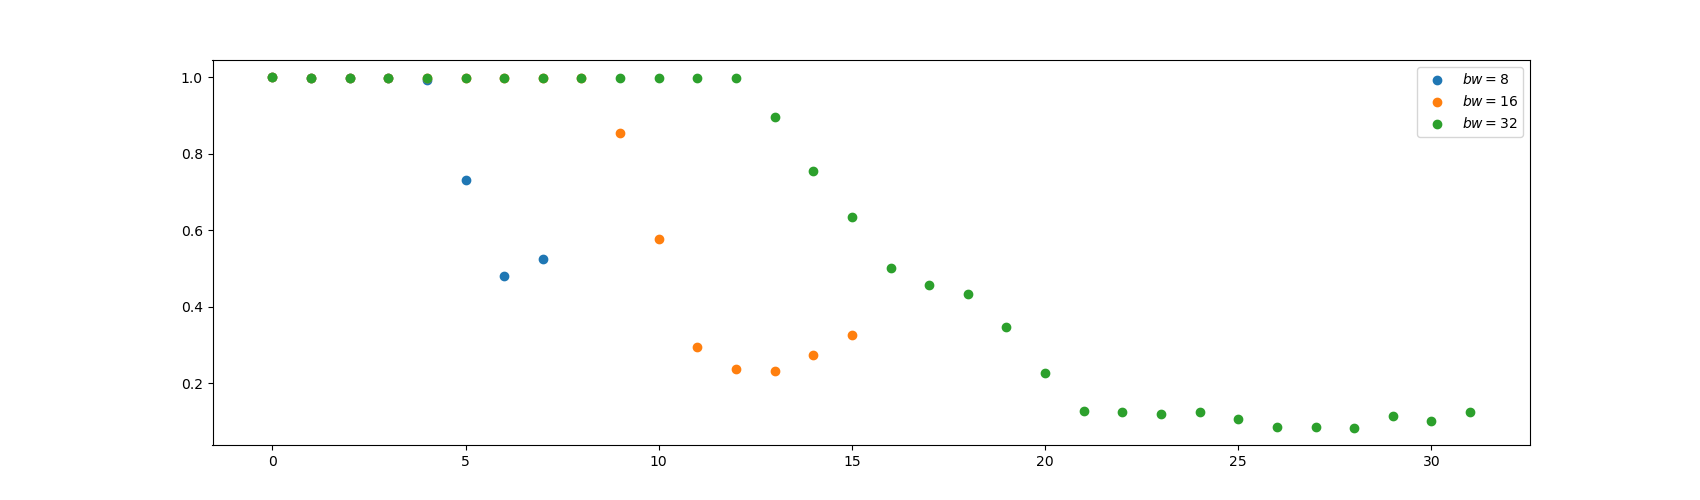
\includegraphics[width=0.9\textwidth]{../codes/03.FEM_laplacian/equiangular/mass_lumping/BL/img/linearFEM_diagonal.png}	
	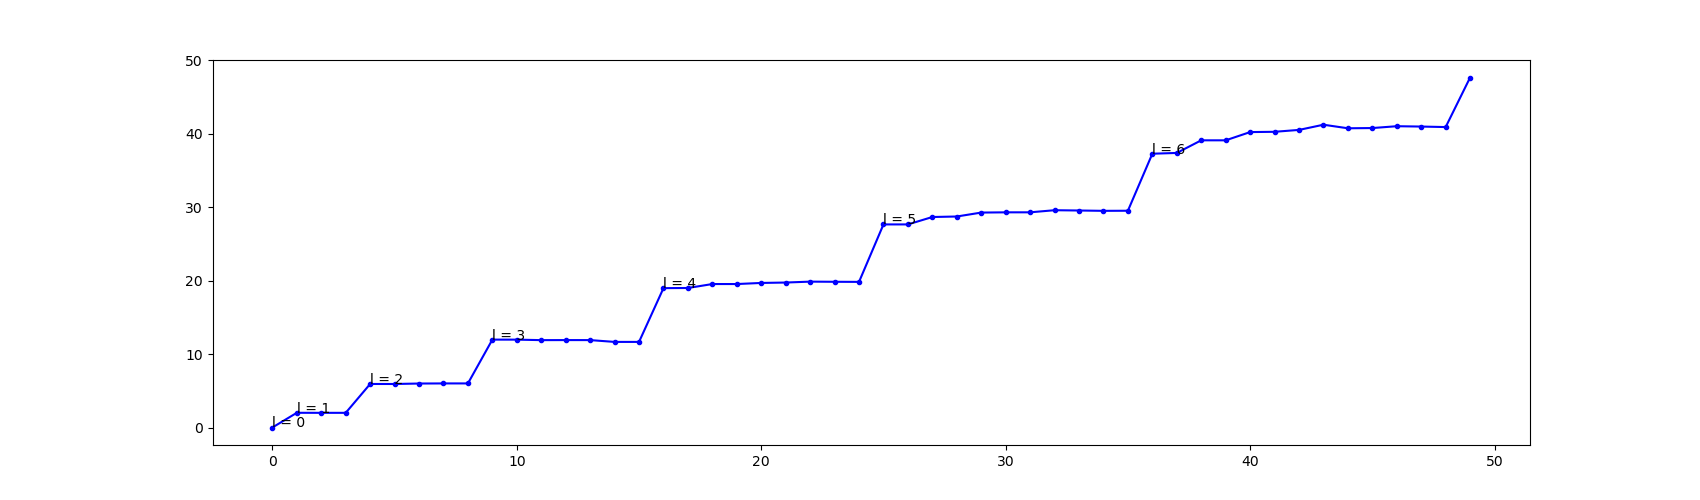
\includegraphics[width=0.9\textwidth]{../codes/03.FEM_laplacian/equiangular/mass_lumping/BL/img/FEM_eigenvalues_32.png}	
\end{figure}

\begin{figure}[h]
	\label{fig:symmetricFEMequiangularLumped}
	\caption{Symmetric Lumped Linear FEM Laplacian on equiangular sampling}
	\centering
	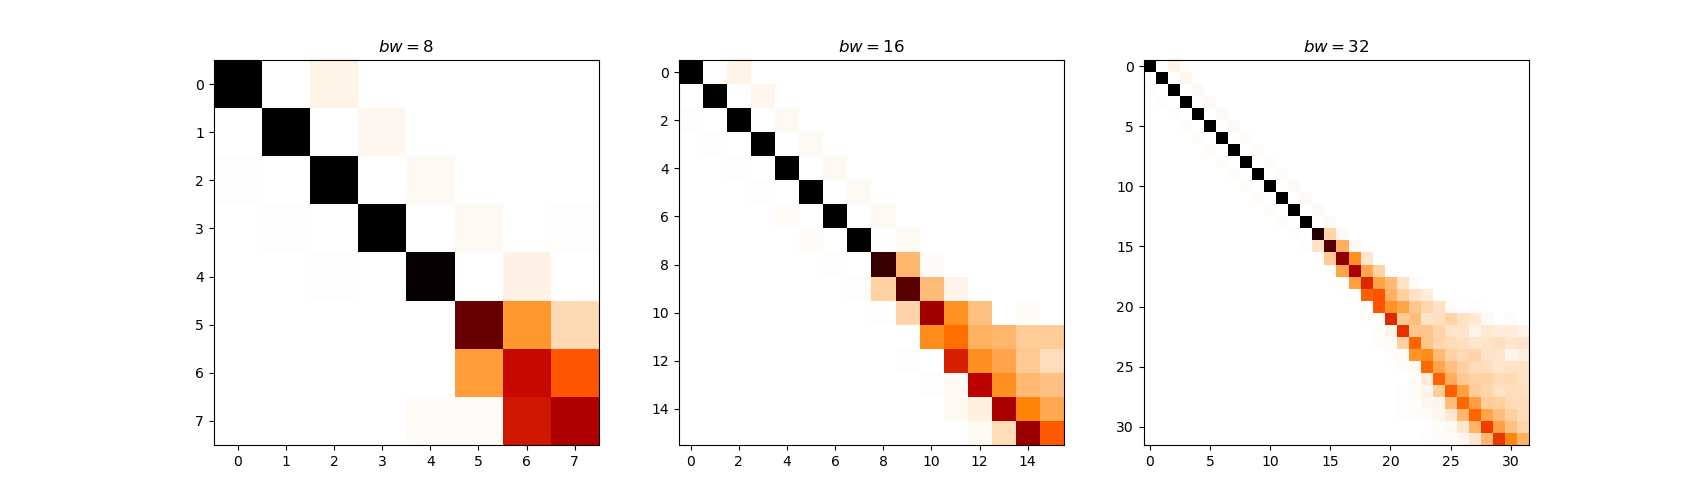
\includegraphics[width=0.9\textwidth]{../codes/03.FEM_laplacian/equiangular/mass_lumping/BLB/img/linearFEM.png}
	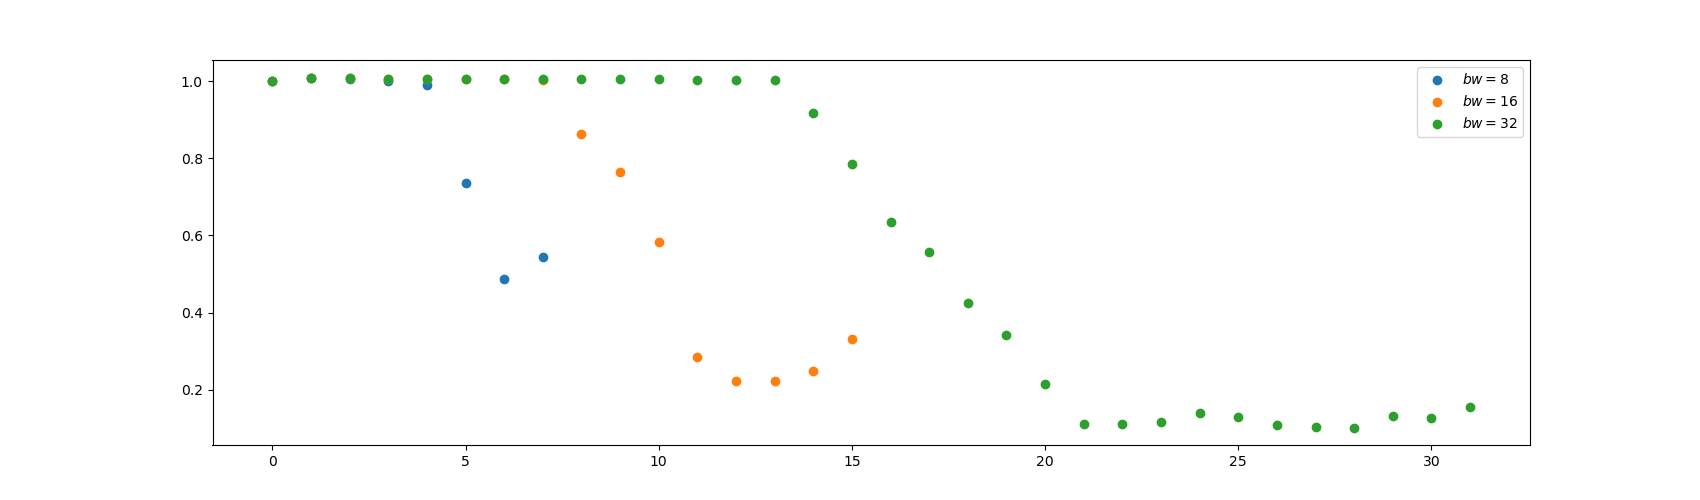
\includegraphics[width=0.9\textwidth]{../codes/03.FEM_laplacian/equiangular/mass_lumping/BLB/img/linearFEM_diagonal.png}	
	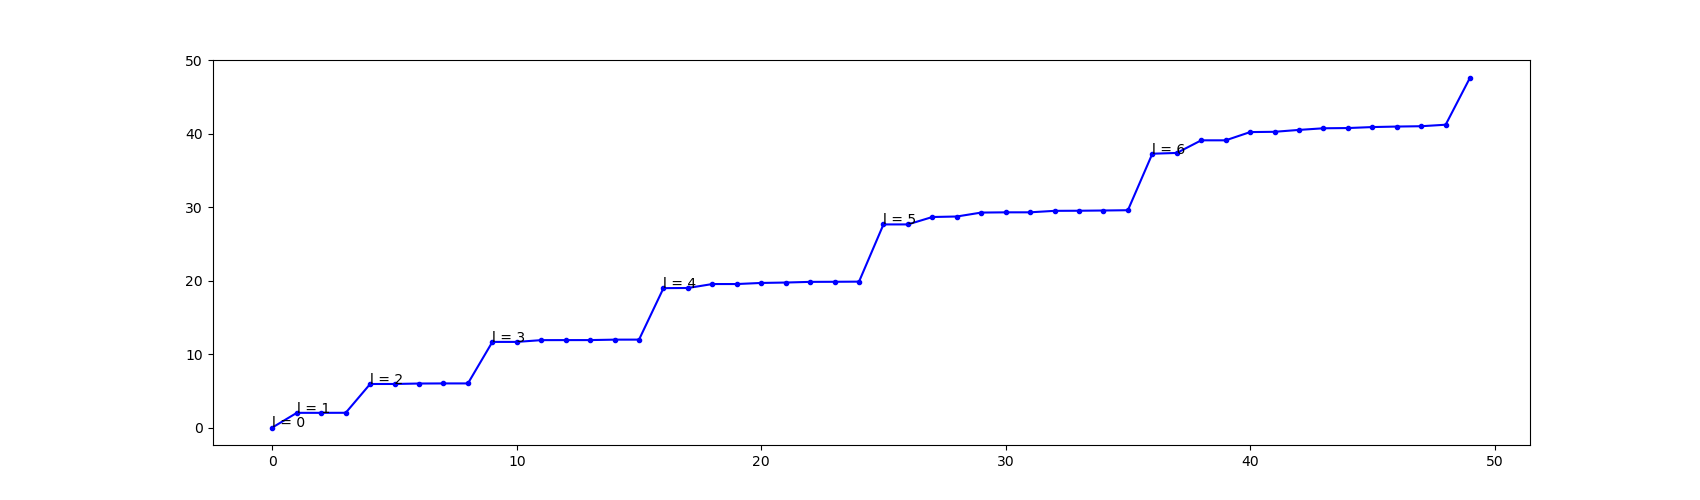
\includegraphics[width=0.9\textwidth]{../codes/03.FEM_laplacian/equiangular/mass_lumping/BLB/img/FEM_eigenvalues_32.png}	
\end{figure}